\documentclass[12pt]{article}
\usepackage[OT1]{fontenc}
\usepackage[utf8]{inputenc}
\usepackage{kpfonts}
\usepackage{graphicx} 
\usepackage[dvipsnames]{xcolor}
\usepackage{amsthm}
\usepackage[margin=1.25in]{geometry}
\usepackage[sf,bf,small,raggedright,compact]{titlesec}
\usepackage[capitalize]{cleveref}
\usepackage{paralist}



\newcommand{\pref}[1]{(P\ref{#1})}
\setlength{\parskip}{1ex}

\newtheorem{thm}{Theorem}
\newtheorem{obs}{Observation}
\newtheorem{lem}{Lemma}

\DeclareMathOperator{\dist}{d}
\DeclareMathOperator{\pack}{pack}
\DeclareMathOperator{\hit}{hit}

\newcommand{\defin}[1]{\emph{\textcolor{Maroon}{#1}}}

\newcommand{\pat}[1]{[\textcolor{red}{#1}]}

\title{Connected Dominating Sets in Triangulations}
\author{Prosenjit Bose \and Vida Dujmović \and Hussein Houdrouge \and Pat Morin \and Saeed Odak \and Anyone Else?}
\date{October 2023}



\begin{document}

\maketitle

% \begin{abstract}
%   We show that every $n$ vertex triangulation $G$ has a spanning tree with at least $n/2\pm{?}$ leaves.  This improves the previous best bound of $2n/5\pm {?}$, due to Kleitman and West (1991). \pat{Is this true? I only find $n/3$.}
% \end{abstract}


\section{Introduction}

A set $X$ of vertices in a graph $G$ is a \defin{dominating set} if each vertex of $G$ is in $X$ or adjacent to a vertex in $X$.  A dominating set $X$ of $G$ is \defin{connected} if the induced graph $G[X]$ is connected.  

% Observe that, for any connected dominating set $X$, $G$ has a spanning-tree in which all vertices in $V(G)\setminus X$ are leaves.  Similarly, by removing the leaves of any spanning tree of $G$ we obtain a tree whose vertex set is a connected dominating set of $G$. 
%  Therefore, an $n$-vertex graph $G$ has a connected dominating set of size $q$ if and only if $G$ has a spanning tree with at least $n-q$ leaves.

\begin{thm}\label{main_result}
  For any $n\ge 4$, any $n$-vertex triangulation $G$ has a connected dominating set of size at most $4n/7 + O(1)$. 
\end{thm}

\section{The Proof}

For a graph $G$, let $|G|=|V(G)|$ denote the number of vertices of $G$.  A \defin{bridge} in a graph $G$ is an edge $e$ of $G$ such that $G-e$ has more connected components than $G$.  A \defin{plane graph} is a graph equipped with a non-crossing embedding in $\mathbb{R}^2$.  A plane graph is \defin{outerplane} if all its vertices appear on the outer face.  A \defin{triangle} is a cycle of length $3$. A \defin{near-triangulation} is a plane graph whose outer face is bounded by a cycle and whose inner faces are all bounded by triangles.  A \defin{generalized near-triangulation} is a plane graph whose inner faces are bounded by triangles.


For a plane graph $H$, we use the notation $B(H)$ to denote the vertex set of the outer face of $H$ and define $I(H):=V(H)\setminus B(H)$.  The vertices in $B(H)$ are \defin{boundary vertices} of $H$ and the vertices in $I(G)$ are \defin{inner vertices} of $H$. For a vertex $v\in B(H)$, the \defin{inner neighbourhood} of $v$ in $H$ is defined as $N_H^+(v):=N_H(v)\cap I(H)$, and the \defin{inner degree} of $v$ in $H$ is $\deg^+_H(v)=|N^+_H(v)|$. 

Let $G$ be a triangulation.  Our procedure for constructing a connected dominating set $X$ begins with an incremental phase that eats away at the triangulation $G$ ``from the outside.'' The process of constructing $X$ is captured by the following definition:   A vertex subset $X\subseteq V(G)$ is \defin{outer-domatic} if it can be partitioned into non-empty subsets $\Delta_0,\Delta_1,\ldots,\Delta_{r-1}$ such that 
\begin{compactenum}[(P1)]
    \item $\Delta_0\subseteq B(G)$; \label{outer_face}
    \item $\Delta_i\subseteq B(G-(\bigcup_{j=0}^{i-1}\Delta_j))$ for each $i\in\{1,\ldots,r-1\}$; and \label{incremental}
    \item $G-(\bigcup_{j=0}^{r-1}\Delta_j)$ is outerplanar. \label{outerplanar}
\end{compactenum} 

\begin{lem}\label{outer_domatic}
    Let $G$ be a triangulation.  Then any outer-domatic $X\subseteq V(G)$ is a connected dominating set of $G$.
\end{lem}

\begin{proof}
  First, suppose $X$ is $f$-domatic and let $\Delta_0,\ldots,\Delta_r$ be the corresponding partition of $X$.  For each $i\in\{1,\ldots,r\}$, let $X_i:=\bigcup_{j=0}^{i-1} \Delta_i$.  First observe that, since $\Delta_0\subseteq B(G)$ is non-empty, $X_i$ contains at least one vertex of $B(G)$, for each $i\in\{1,\ldots,r\}$. We claim that
  \begin{compactenum}[(P1)]\setcounter{enumi}{3}
    \item each vertex in $B(G-X_{i-1})$ is adjacent to some vertex in $X_{i-1}$, for each $i\in\{2,\ldots,r\}$. \label{adjacent} 
  \end{compactenum} 
  Indeed, for any $i\in\{2,\ldots,r\}$ and any vertex $v\in B(G-X_{i-1})$ is either in $B(G)$ or adjacent to a vertex in $X_{i-1}$. Even in the former case $v$ is adjacent to a vertex in $X_1=\Delta_0\subseteq X_{i-1}$, because because $G[B(G)]$ is a clique.

  We now prove, by induction on $i$, that $G[X_i]$ is connected, for each $i\in\{1,\ldots,r\}$.
  The fact that $G[B(G)]$ is a clique and \pref{outer_face} implies that $G[X_1]=G[\Delta_0]$ is connected. For each $i\in\{2,\ldots,r\}$, the assumption that $G[X_{i-1}]$ is connected, \pref{incremental}, and \pref{adjacent} then imply that $G[X_i]=G[X_{i-1}\cup\Delta_{i-1}]$ is connected.  
  
  In particular $G[X_r]=G[X]$ is connected.  Finally, \pref{adjacent}, with $i=r$ and \pref{outerplanar} implies that $N_G(X_r)=B(G-X_r)=V(G-X_r)$, so $X_r=X$ is a dominating set of $G$.
\end{proof}

We will present two algorithms that grow a connected dominating in small batches $\Delta_0,\Delta_1,\ldots,\Delta_{r-2}$ that result in a sequence of sets $X_1,\ldots,X_{r-1}$ where $X_{i}=\bigcup_{j=0}^{i-1}\Delta_j$.  However, each of these algorithms is unable to continue once they reach a point where each vertex in $B(G-X_i)$ has inner-degree at most $1$ in $G-X_i$.  We begin by studying the graphs that cause this to happen.

\subsection{Critical Graphs}

A generalized near-triangulation $H$ is \defin{critical} if $\deg^+_H(v)\le 1$ for each $v\in B(H)$.


\begin{lem}\label{base_case}
    Let $H$ be critical generalized near-triangulation. Then $|B(H)|\ge 3|I(H)|$ and there exists $\Delta\subseteq B(H)$ of size at most $|I(H)|$ that dominates $I(H)$. 
\end{lem}

\begin{proof}
  Let $B:=B(H)$ and $I:=I(H)$.  If $I$ is empty then the result is trivially true, by taking $X:=\emptyset$, so we now assume that $I$ is non-empty.  By definition, the graph $H[B]$ is outerplanar.  Say that an inner face of $H[B]$ is \defin{marked} if it contains an inner vertex of $H$.  Consider some marked face $f$ of $H[B]$.  This face is marked because it contains at least one vertex in $I$.  Since $G$ is a triangulation, there is an edge $vx$ in $G$ with $v\in B$ on the boundary of $f$ and $x\in I$ in the interior of $f$.  The vertex $v$ is incident to an edge $vw$ on the boundary of $f$. By the same reasoning $G$ contains an edge $wx'$ with $x'\in I$ in the interior of $f$.  Therefore $\deg^+_H(v),\deg^+_H(w)\ge 1$ and since $H$ is critical, $\deg^+H(v)=\deg^+_H(w)=1$.  Since $G$ is a triangulation the triangle $vwx$ is a face of $G$ and the triangulation $vwx'$ is a face of $G$.  Since $\deg^+H(v)=\deg^+_H(w)=1$, $x=x'$.  We can make this argument for each edge of $f$ to conclude that $f$ contains exactly one vertex $x_f$ of $I$ and $x_f$ is adjacent to each vertex of $f$.  Thus, $H$ is formed from an outerplanar graph $H[B]$ by adding $|I|$ stars, one in the interior of each marked face of $H[B]$.  Furthermore, since $\deg_H^+(v)=1$ for each $v\in B$, each vertex of $H[B]$ is on the boundary of exactly one marked face.

    \begin{figure}
        \begin{center}
            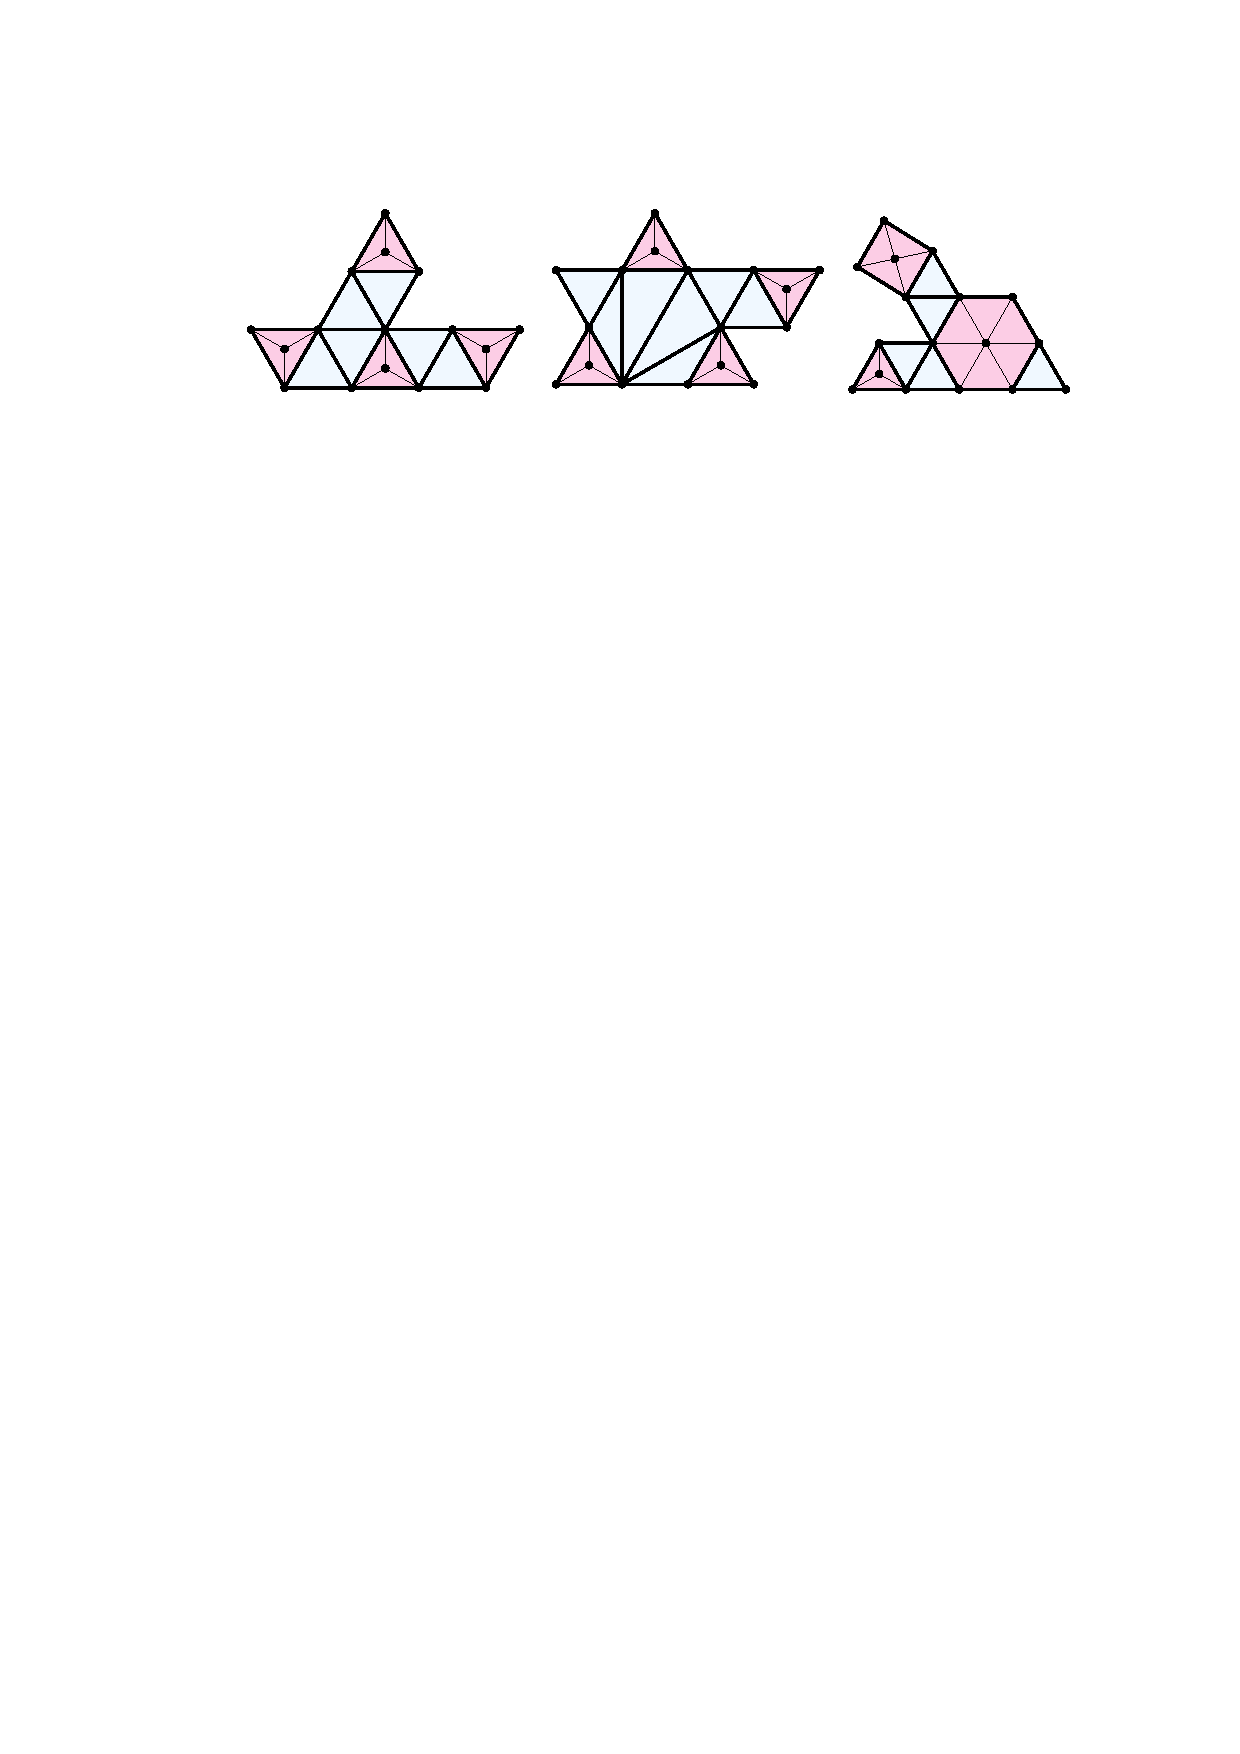
\includegraphics[page=1]{figs/critical} \\
            % \includegraphics[page=2]{figs/critical} \\
        \end{center}
        \caption{Some critical graphs \pat{Add some examples where $H[B(H)]$ has some non-triangular faces}}
        \label{critical_fig}
    \end{figure}
    
  Consider the graph $H'$ obtained by adding edges to the inner faces of $H[B]$ so that each inner face is a triangle. For each marked face $f$ of $H[B]$, select one triangular face $t_f$ of $H'$ that is contained in $f$ and \defin{mark} $t_f$.  Observe that the three vertices of $t_f$ are all adjacent, in $G$ to $x_f$.  Thus there is a bijection from the set of marked faces of $H[B]$ to the set of marked faces in $H'$ and both of these sets have size $|I|$.  Since each vertex in $B$ is on the boundary of at most one marked face of $H[B]$, each vertex in $B$ is on the boundary of at most one marked triangular face of $H'$.  Therefore, $|B| \ge 3|I|$ so $|H|=|B|+|I|\ge 4|I|$.  By choosing one vertex from each marked triangular face of $H'$ we obtain the desired set $\Delta$. 
\end{proof}


\section{A Simple Algorithm}

% We will construct a sequence of vertex sets $\emptyset = X_0\subsetneq X_1\subsetneq\cdots\subsetneq X_r$ such that $G[X_i]$ is connected for each $i\in\{1,\ldots,r\}$ and $X_r$ dominates $G$.  Let $G_0:=G$, let $D_0:=B_0:=B(G_0)$, and let $I_0:=V(G_0-D_0)$. For each $i\in\{1,\ldots,r\}$, let $D_i:=N_G[X_i]$, let $I_i:=V(G-D_i)$, let $B_i:=N_G(I_i)$, let $\Delta_{i-1}:=X_{i}\setminus X_{i-1}$, and let $G_i:=G[I_i\cup B_i]$.  


% In words, $D_i$ contains all the vertices that are dominated by $X_i$; $I_i$ contains the vertices that are not dominated by $X_i$; $B_i$ contains all the vertices on the boundary between $X_i$ and $I_i$ (each vertex in $B_i$ is adjacent to at least one vertex in $X_i$ and at least one vertex in $I_i$); and $\Delta_i$ is the set of vertices we add to $X_i$ to get $X_{i+1}$. These sets will obey the following conditions:
% \begin{compactenum}[(P1)]
%     \item $\Delta_i\subseteq B_i$, for each $i\in\{0,\ldots,r-1\}$; 
%     \item $G_r$ is outerplane. 
% \end{compactenum}

We start with the simplest imaginable greedy algorithm, that we call $\textsc{SimpleGreedy}(G)$, to choose $\Delta_0,\ldots,\Delta_{r-1}$.  Suppose we have already chosen $\Delta_0,\ldots,\Delta_{i-1}$ for some $i\ge 0$ and we now want to choose $\Delta_i$.  Let $X_i:=\bigcup_{j=0}^{i-1}\Delta_j$, let $G_i:=G-X_i$, and let $v_i$ be a vertex in $B(G_i)$ that maximizes $\deg^+_{G_i}(v_i)$.  During iteration $i\ge 0$, there are only two cases to consider:  
\begin{compactenum}
    \item If $\deg^+_{G_i}(v_i)\ge 2$ then we set $\Delta_i\gets\{v_i\}$.
    \item If $\deg^+_{G_i}(v_i)\le 1$ for all $v\in G_i$ then $G_i$ is critical and this is the final step, so $r:=i+1$.  By \cref{base_case}, there exists $\Delta_i\subseteq B_i$ of size at most $|I_i|$ that dominates $I_i$. Then $X_r:=X_{r-1}+\Delta_{i}$ and we are done.
\end{compactenum}

\begin{thm}\label{simple_greedy}
  When applied to an $n$-vertex triangulation $G$,  $\textsc{SimpleGreedy}(G)$ produces a connected dominating set $X_r$ of size at most $(4n+6)/7$.
\end{thm}

\begin{proof}
By the choice of $\Delta_0,\ldots,\Delta_{r-1}$, $X_r$ is an outer-domatic subset of $V(G)$ so, by \cref{outer_domatic}, $X_r$ is a connected dominating set of $G$.  All that remains is to analyze the size of $X_r$.  For each $i\in\{1,\ldots,r\}$, let $D_i:=N_G(X_i)$ be the subset of $V(G)$ that is dominated by $X_i$, let $I_i:=V(G)\setminus D_i$ be the subset of $V(G)$ not dominated by $X_i$, and let $B_i:=N_G(I_i)$ be the vertices of $G$ that have at least one neighbour in each of $X_i$ and $I_i$.  We use the convention that $D_0:=B(G)$.

First observe that, for $i\in\{0,\ldots,r-2\}$, $|D_{i+1}|\ge |D_i|+\deg_{G_i}^+(v_i)$ since $D_{i+1}\supseteq D_i$ and $D_{i+1}$ contains the $\deg_{G_i}^+(v_i)$ inner neighbours of $v_i$ in $G_i$.  Therefore
\[
    |D_{r-1}| \ge |D_0| + \sum_{i=0}^{r-2} \deg_{G_i}^+(v_i) \ge 3 + \sum_{i=0}^{r-2} 2 =  2r+1 \enspace . \label{double_d}
\]
Since $D_{r-1}$ and $I_{r-1}$ partition $V(G)$, 
\begin{equation}
  n = |D_{r-1}| + |I_{r-1}| \ge 2r+1 + |I_{r-1}|  \enspace . \label{c1}
\end{equation}
% so
% \begin{equation}
%     r\le \frac{n-|I_{r-1}|-1}{2}  \enspace . 
% \end{equation}

Since $X_{r-1}$ and $B_{r-1}$ are disjoint and $D_{r-1}\supseteq B_{r-1}\cup X_{r-1}$, we have $|D_{r-1}|\ge |X_{r-1}| + |B_{r-1}|=r-1+|B_{r-1}|$.  Therefore, 
\begin{equation}
    n = |D_{r-1}| + |I_{r-1}| \ge r-1 + |B_{r-1}| + |I_{r-1}| = r-1 + |B_{r-1}| + |I_{r-1}|
    \ge r - 1 + 4|I_{r-1}| \enspace , \label{c2}
\end{equation}
where the last inequality follows from \cref{base_case}.  

The final dominating set $X_r$ has size $|X_r| = |X_{r-1}| + \Delta_{r-1} = r - 1 +|I_{r-1}|$, so the size of $|X_r|$ can be upper-bounded by maximizing $r+|I_{r-1}|$ subject to the constraints \cref{c1,c2}.  More precisely, the maximum size of $X_r$ is upper bounded by the maximum value of $x-1+y$ subject to the constraints
\begin{align*}
  x - 1 + 4y & \le n \\
  2x + y +1 & \le n
\end{align*}

% r\le (n+1-I_{r-1})/2$ and $r+4|I_{r-1}|\le n$.  
This is an easy linear programming exercise and the maximum value of $X_{r}$ is obtained when $r=(3n-5)/7$ and $|I_{r-1}|=(n+3)/7$, which gives
$|X_r| \le (4n-9)/7$.
\end{proof}

\section{A Less Simple Algorithm}

Next we devise an algorithm that produces a smaller connected dominating set than what is guaranteed by $\textsc{SimpleGreedy}(G)$.  This involves a more careful analysis of the cases in which \textsc{SimpleGreedy} is forced to take a vertex $v_i$ with $\deg^+_{G_i}(v_i)=2$.  We begin by identifying unnecessary vertices and edges that can appear in the graphs $G_1,\ldots,G_{r-1}$ during the construction of $X$.   We say that a near-triangulation $H$ is \defin{dom-minimal} if
\begin{compactenum}[({DM}1)]
    \item $\deg^+_H(v)\ge 1$ for each $v\in B(H)$; and \label{bad_vertex} 
    \item $vw$ is on the boundary of an inner face $vwx$ for some $x\not\in B(H)$, for each edge $vw\in G[B(H)]$. \label{bad_edge}
\end{compactenum}
We say that a generalized near-triangulation $H$ is \defin{dom-minimal} if each of its biconnected components are dom-minimal. 

\begin{obs}
    Any dom-minimal generalized near-triangulation $H$ is bridgeless.
\end{obs}

\begin{proof}
   If $vw$ is a bridge in $H$ then both $v$ and $w$ are in $B(H)$.  Since $vw$ is a bridge in $H$, there is no inner face $vwx$ in $H$. Thus $H$ does not satisfy the second condition for dom-minimality.
\end{proof}

A subgraph $H'$ of a generalized near-triangulation $H$ is \defin{dom-preserving} if
\begin{compactenum}[({DP}1)]
  \item $B(H')\subseteq B(H)$;
  \item $N^+_{H'}(v)=N^+_H(v)$ for all $v\in B(H')$;
  \item $I(H')=I(H)$; and 
  \item $N_{H'}(v)=N_H(v)$ for all $v\in I(H)$.
\end{compactenum} 

\begin{obs}
  Let $H$ be a generalized near-triangulation, let $H'$ be a dom-preserving subgraph of $H$, and let $\Delta$ be a subset of $V(H)$ that dominates $I(H)$.  Then $\Delta\cap V(H')$ dominates $I(H)$.    
\end{obs}

\begin{proof}
  Each vertex $v\in I(H')$ is adjacent to some vertex $w\in \Delta$.  Since $N_{H'}(v)=N_H(v)$, $w\in\Delta\cap V(H')$, so $v$ is dominated by $\Delta\cap V(H')$.  Since this is true for each $v\in I(H)=I(H')$, $\Delta\cap V(H')$ dominates $I(H)$.    
\end{proof}

\begin{lem}\label{dom-minimal}
  For any generalized near-triangulation $H$, there exists a dom-preserving subgraph $H'$ of $H$ that is dom-minimal. 
\end{lem}

\begin{proof}
  The proof is by induction on $|V(H)|+|E(H)|$.  If $H$ is already dom-minimal, then setting $H'=H$ satisfies the requirements of the lemma, so assume that $H$ is not dom-minimal.  It is straightforward to verify that the dom-preserving subgraph relationship is transitive, so if $H$ has a dom-preserving subgraph $H^*$ and $H^*$ has a dom-preserving subgraph $H'$ then $H'$ is a dom-preserving subgraph of $H$.  Therefore, it is sufficient to show the existence of a dom-preserving subgraph $H^*$ of $H$ with fewer edges or fewer vertices than $H$, and the inductive hypothesis provides the desired dom-minimal dom-preserving subgraph $H'$ of $H$.
  
  If $H$ contains a vertex $v\in B(H)$ with $\deg^+_H(v)=0$ then $H-v$ is a dom-preserving subgraph of $H$ with fewer vertices than $H$.  We now assume that $\deg^+_H(v)\ge 1$ for all $v\in B(H)$.
  
  Since $H$ is not dom-minimal then $H$ contains a biconnected component $C$ that is not dom-minimal.  
  \begin{compactenum}
    \item If there exists an edge $vw$ on the outer face of $C$ that is not incident to any inner face $vwx$ with $x\in I(C)$ then $B(H-vw)=B(H)$ and $I(H-vw)=I(H)$, and $H-vw$ is a is dom-preserving subgraph of $H$ that has fewer edges than $H$.

    \item If there exists a vertex $v\in B(C)$ with $\deg^+_C(v)=0$ then $v$ is incident to an edge $vw$ that is on the outer face of $C$ and on the outer face of $H$. Since $\deg^+_C(v)=0$, $vw$ is not incident to any inner face $vwx$ with $x\in I(C)$ and we can proceed as in the previous case. \qedhere
  \end{compactenum}
\end{proof}

We say that a generalized near-triangulation $H$ is \defin{good} if 
\begin{compactenum}[(G1)]
      \item $H$ is critical;
      \item there exists $v\in B(H)$ with $\deg^+_H(v)\ge 3$; or
      \item there exists distinct $v,w\in B(H)$ such that $\deg^+_H(v)=2$ and $N^+_H(w)\subseteq N^+_H(v)$.
\end{compactenum}

\begin{lem}\label{not_good}
  Let $H$ be a dom-minimal generalized near-triangulation.  Then \begin{compactenum}[(i)]
    \item $H$ is good or 
    \item $B(H)$ contains a vertex $v$ with $\deg^+_H(v)=2$ such that $G-v$ is good.
  \end{compactenum}
\end{lem}

\begin{proof}
  Since $H$ is dom-minimal, each vertex in $B(H)$ has inner-degree greater than $0$.  If some vertex in $B(H)$ has inner-degree at least $3$ then $H$ is good and there is nothing to prove, so we may assume that each vertex in $B(H)$ has inner-degree $1$ or $2$.  Since $H$ is not critical, at least one vertex in $B(H)$ has inner-degree $2$.

  If $H$ is $2$-connected, let $C:=H$ and let $v_0$ be any vertex of $H$ with inner-degree $2$.  
  If $H$ is not $2$-connected, then let $C$ be a biconnected component of $H$ that contains a single cut-vertex $v_0$ of $H$ (so $C$ is a leaf in the block-cut tree of $H$). Then $v_0$ is contained in a second biconnected component $C'\neq C$ of $H$. Since $H$ is dom-minimal, $\deg^+_{C}(v_0)\ge 1$ and $\deg^+_{C'}(v_0)\ge 1$, so $\deg^+_H(v)= 2$.

  Since $C$ is biconnected its outer face is bounded by a cycle $v_0,v_1,v_2,\ldots,v_{k-1}$.  From this point on, all subscripts on $v$ are taken modulo $k$.  If $\deg^+_C(v_1)=1$ then, since $H$ is dom-minimal, the edge $v_0v_1$ is on the boundary of an inner face $v_0v_1x$ with $x\in I(H)$.  Since $v_0$ is the only cut-vertex of $H$ in $C$, $N^+_H(v_1)=N^+_C(v_1)=\{x\}\subseteq N_H(v_0)$ and $\deg^+_H(v_0)=2$, so $H$ is good and there is nothing to prove.  We now assume that $\deg^+_C(v_1)=2$.  By the same reasoning, we may assume that $\deg^+_C(v_i)=2$ for each $i\in\{1,\ldots,k-1\}$.  (Otherwise, $N^+_H(v_i)\subseteq N^+_H(v_{i-1})$ and $\deg^+_H(v_{i-1})=2$ for some $i\in\{2,\ldots,k-1\}$ and $H$ is good.)

  To summarize, so far we know that some vertex $x\in I(H)$ is in $N^+_H(v_0)$, $N^+_H(v_1)$, and $N^+_H(v_{k-1})$.  If $k=3$ then, since $H$ is dom-minimal, $H$ contains a face $v_1v_{k-1}y$ with $y\in I(H)$.  Since $\deg^+_H(v_1)=\deg^+_H(v_{k-1})=2$, $y\neq x$ and $N^+_H(v_1)=N^+_H(v_2)=\{x,y\}$. Again, this implies that $H$ is good.  If $k\ge 5$, then consider the graph $H':=H-v_0$.  Then $\deg^+_{H'}(v_1)=1$, $\deg^+_{H'}(v_2)=2$, and $N_{H'}(v_1)\subseteq N_{H'}(v_2)$.   Therefore $G'$ is good, so $G$ contains a vertex $v=v_0$ of inner-degree $2$ such that $G-v$ is good.  This completes the proof.
\end{proof}


This gives variant of the $\textsc{SimpleGreedy}(G)$ that we call $\textsc{BetterGreedy}(G)$.  Suppose we have already chosen $\Delta_0,\ldots,\Delta_{i-1}$ for some $i\ge 0$ and we now want to choose $\Delta_i$.  Let $X_i:=\bigcup_{j=0}^{i-1}\Delta_j$, let $G_i$ be a dom-preserving subgraph of $G-X_i$ that is dom-minimal, and let $v_i$ be a vertex in $B(G_i)$ that maximizes $\deg^+_{G_i}(v_i)$.  During iteration $i\ge 0$, there are only two cases to consider:  
\begin{compactenum}
    \item If $\deg^+_{G_i}(v_i)\ge 3$ then we set $\Delta_i\gets\{v_i\}$.
    \item If there exists distinct $v_i,w\in B(H)$ such that $\deg^+_H(v)=2$ and $N^+_H(w)\subseteq N^+_H(v)$ then set $\Delta_i:=\{v_i\}$.
    \item If $\deg^+_{G_i}(v_i)\le 1$ for all $v\in G_i$ then $G_i$ is critical and this is the final step, so $r:=i+1$.  By \cref{base_case}, there exists $\Delta_i\subseteq B_i$ of size at most $|I_i|$ that dominates $I_i$. Then $X_r:=X_{r-1}+\Delta_{i}$ and we are done.
    \item Otherwise, $G_i$ is not good.  By \cref{not_good}, $G$ contains a vertex $v_i$ such that $G-v_i$ is good.  Set $\Delta_i:=\{v_i\}$.
\end{compactenum}

\begin{thm}\label{better_greedy}
  When applied to an $n$-vertex triangulation $G$,  $\textsc{BetterGreedy}(G)$ produces a connected dominating set $X_r$ of size at most $10n/19\pm{?}$.
\end{thm}

\begin{proof}
  Let $x_2$ be the number of times $\textsc{BetterGreedy}(G)$ falls into Case~4.
  For each integer $t\ge 3$, let $x_t$ be the number of times $\textsc{BetterGreedy}(G)$ falls into case $1$ and chooses $v_i$ such that $\deg^+_{G_i}(v_i)=t$.  Let $z$ be the number of times $\textsc{BetterGreedy}(G)$ falls into Case~2.  From \cref{not_good}, we know that
  \begin{equation}
      x_2 \le \sum_{t\ge 3}x_t + z \enspace .
  \end{equation}
  The size of the dominated set $D_{r-1}$ is at least
  \[
    |D_{r-1}| \ge 3 + \sum_{t\ge 2}tx_t + 2z 
  \]
  The size of the boundary $B_{r-1}$ is at most
  \begin{equation}
       |B_{r-1}| \le 3 + \sum_{t\ge 2} (t-1)x_t \\
  \end{equation}
  By definition,
  \[
     r-1 = |X_{r-1}| = \sum_{t\ge 2} x_t + z 
  \]
  As in the previous proof, we combine these constraints with the constraints $n=|D_{r-1}|+|I_{r-1}|$,  $|D_{r-1}|\ge r-1+|B_{r-1}|$ and $|D_{r-1}|\ge r-1+3|I_{r-1}|$.

  Here is an approximation of this in Sage:
  \begin{verbatim}
p = MixedIntegerLinearProgram()
v = p.new_variable()
D, I, B, r, n, x2, x3, x4, x5, x12 = v["D"], v["I"], v["B"], v["r"], v["n"], v["x2"], v["x3"], v["x4"], v["x5"], v["x12"]
N = 1000000000
p.add_constraint(n <= N)
p.add_constraint(x2 >= 0)
p.add_constraint(x3 >= 0)
p.add_constraint(x4 >= 0)
p.add_constraint(x5 >= 0)
p.add_constraint(x12 >= 0)
p.add_constraint(D + I == n)
p.add_constraint(D >= 3 + 2*x2 + 3*x3 + 4*x4 + 5*x5 + 2*x12)
p.add_constraint(r - 1 == x2 + x3 + x4 + x5 + x12)
p.add_constraint(B <= 3 + x2 + 2*x3 + 3*x4 + 4*x5)
p.add_constraint(x2 <= (x3 + x4 + x5 + x12 + 1)/2)
p.add_constraint(D >= r - 1 + B)
p.add_constraint(B >= 3*I)
p.set_objective(r - 1 + I)
ds = p.solve()
print("n={}, sol={}n, sol-10/19={:.20f}".format(N, ds/N, ds/N - 10/19))
sol = p.get_values(v)
print(sol)
  \end{verbatim}
  and we get the output:
  \begin{verbatim}
      n=1000000000, sol=0.5263157884210526n, sol-10/19=-0.00000000105263153749
{'D': 947368420.1578947, 'I': 52631579.84210527, 'B': 157894739.5263158, 'r': 473684209.57894737, 'n': 1000000000.0, 'x2': 157894736.5263158, 'x3': -0.0, 'x4': -0.0, 'x5': -0.0, 'x12': 315789472.05263156}

  \end{verbatim}
  %   & = 3 + 2x_2+2z+\sum_{t\ge 3}(t-1)tx_t + x_{\ge 3} \\
  %   & \ge 3 + x_2 + 2z + |B_{r-1}| + x_{\ge3} \\
  %   & \ge 3 + x_2 + 2z + |B_{r-1}| + x_{\ge3} \\
  %   % & \ge 3 + 2x_2 + 2z + 3|I_{r-1}| + x_{\ge3} \\
  %   % & \ge 3 + 2x_2 + 2z + \sum_{t\ge 3}2x_t + x_{\ge3} \\
  %   % & = 1 + 2(x_2+ z+x_{\ge 3}) + x_{\ge3} \\
  %   % & \ge 3 + 2(x_2+z)+3x_{\ge 3}  \\
  %   % & = 3 + 2(x_2+z)+3(r-1-x_2-z) & \text{(since $x_{\ge 2}+z=r-1$)} \\
  %   % & = 3r - x_2 - z  \\
  %   % & \ge 3r - r/2 - z  & \text{(since $x_2\le r/2$)}\\
  %   % & \ge 5r/2 - z  & \text{(since $x_2\le r/2$)}\\
  %   % \enspace .
  % \end{align*}
  % Since $|D_{r-1}|+|I_{r-1}|=n$, this gives
  % \begin{equation}
  %   3 + 2x_2 + 2z + \sum_{t\ge 3}tx_t + |I_{r-1}| \le n
  % \end{equation}
  % By definition,
  % \[
  %    r-1 = |X_{r-1}| = x_2 + \sum_{t\ge 3} x_t + z 
  % \]
  % As before, we have
  % \[
  %    |B_{r-1}| \ge 3|I_{r-1}|
  % \]
  % but now we also have
  % \begin{align*}
  %    |B_{r-1}| & \le 3 + \sum_{t\ge 2} (t-1)x_t \\
  %    & = 3 + \sum_{t\ge 2} tx_t - (r-1) \\
  %    & = 3 + \sum_{t\ge 2} tx_t - (r-1) \\
  %    & \le |D_{r-1}| - 2z -(r-1)
  %    \enspace .
  % \end{align*}
  % Therefore,
  % \[
  % 3|I_{r-1}| \le |B_{r-1}| \le 3 + \sum_{t\ge 2} (t-1)x_t
  % = -r+4 + \sum_{t\ge 2} tx_t
  % \]
  % Since $|D_{r-1}|\ge |X_{r-1}|+|B_{r-1}|=r-1+|B_{r-1}|$ the identity $|D_{r-1}|+|I_{r-1}|=n$ gives
  % \[
  %    3 + \sum_{t\ge 2} tx_t + |I_{r-1}| \le n
  % \]
  Now we just need to solve the actual LP by hand to get a rigorous proof.  This is a little bit annoying because we have infinitely many variables $x_t$, $t\ge 2$, but $x_t$ seems to be redundant for all $t\ge 3$.
\end{proof}


\end{document}


% At all times we will be working with a near triangulation $G$ that was obtained by removing vertices from a starting triangulation $G_0$ and we have already constructed a connected dominating set $X_0\subseteq V(G_0)\setminus V(G)$ for the graph $G_0-(V(G)\setminus L(G))$. Thus, the vertices of $L(G)$ are dominated by $X_0$ but are not contained in $X_0$.  Our next step will be to remove one or more vertices from $L(G)$ with choice made based on $\deg^+_G(v)$.  If we simply remove one vertex $v$ from $L(G)$ and put it in $X_0$ then the size of $X_0$ increases by $1$ and the number of vertices dominated by $X_0$ increases by $\deg^+_G(v)-1$.  Thus, in order to keep the number of vertices dominated by $X_0$ at least as large as the number of vertices in $X_0$ we would like to remove a vertex $v$ with $\deg_G^+(v)\ge 2$. Therefore, we first characterize the cases where this is not possible.

% If $L(G)$ contains a vertex $v$ with $\deg_G^+(v)=0$, then we can simply apply induction on $G-v$.....

% \subsection{Basic Graphs}

% For ease of notation, let $G=G_i$ and suppose that $\deg_G^+(v)=1$ for each $v\in L(G)$.  Consider the induced subgraph $H:=G[L(G)]$.  Then $H$ is outerplanar because it is a subgraph of $G$ that only contains vertices on the outer face of $G$.  

% % Suppose that $H$ contains a cut vertex $v$ and let $G_0$ and $G_1$ be two subgraphs of $G$ whose union is $G$ and whose intersection is the vertex $v$.  Since $\deg^+G(v)=1$, exactly one of these subgraphs, say $G_0$, has $\deg_G^+(v)=1$ and the other, $G_1$ has $\deg_G^+(v)=0$.  Then any component of $G[X]$ that contains vertices of $G_1-v$ intersects $L(G_1-v)$, so we can treat induction on $G_0$ and $G_1-v$.  Therefore, we may assume that $H$ contains no cut vertices, so $H$ is $2$-connected.

% Since $\deg_G^+(v)=1$ for each $v\in L(G)=V(H)$, $N_G(v)\setminus L(G)$ contains exactly one vertex $x_v$ in the interior of exactly one inner face $f_v$ of $H$.  Now consider some face $f$ of $H$ and the set $I_f:=\{v\in V(H):f_v = f\}$.  If $I_f$ is empty then, since $G$ is a triangulation, $f$ is a triangle.  If $I_f$ is non-empty, then each edge $vw$ of $f$ is incident to some triangle $vwx$ contained in $f$.  Therefore $x_v=x_w=x$.  Therefore, each face $f$ of $H$ is either a triangle formed by three vertices of $L(G)$ and containing no vertices of $G-L(G)$ in its interior or $f$ contains a single vertex $x_f$ of $G$ in its interior, and $x_f$ is adjacent to all vertices of $f$.  In the latter case, we call $f$ a \defin{marked face} of $H$.  Since $\deg_G^+(v)=1$ for all $f$, each vertex of $H$ is incident to exactly one marked face of $H$.  We call a graph $G$ of this kind, a \defin{basic graph}.  We say that the basic graph $G$ is \defin{critical} if each marked face of $G[L(G)]$ is a triangle.

% \begin{figure}
%     \begin{center}
%         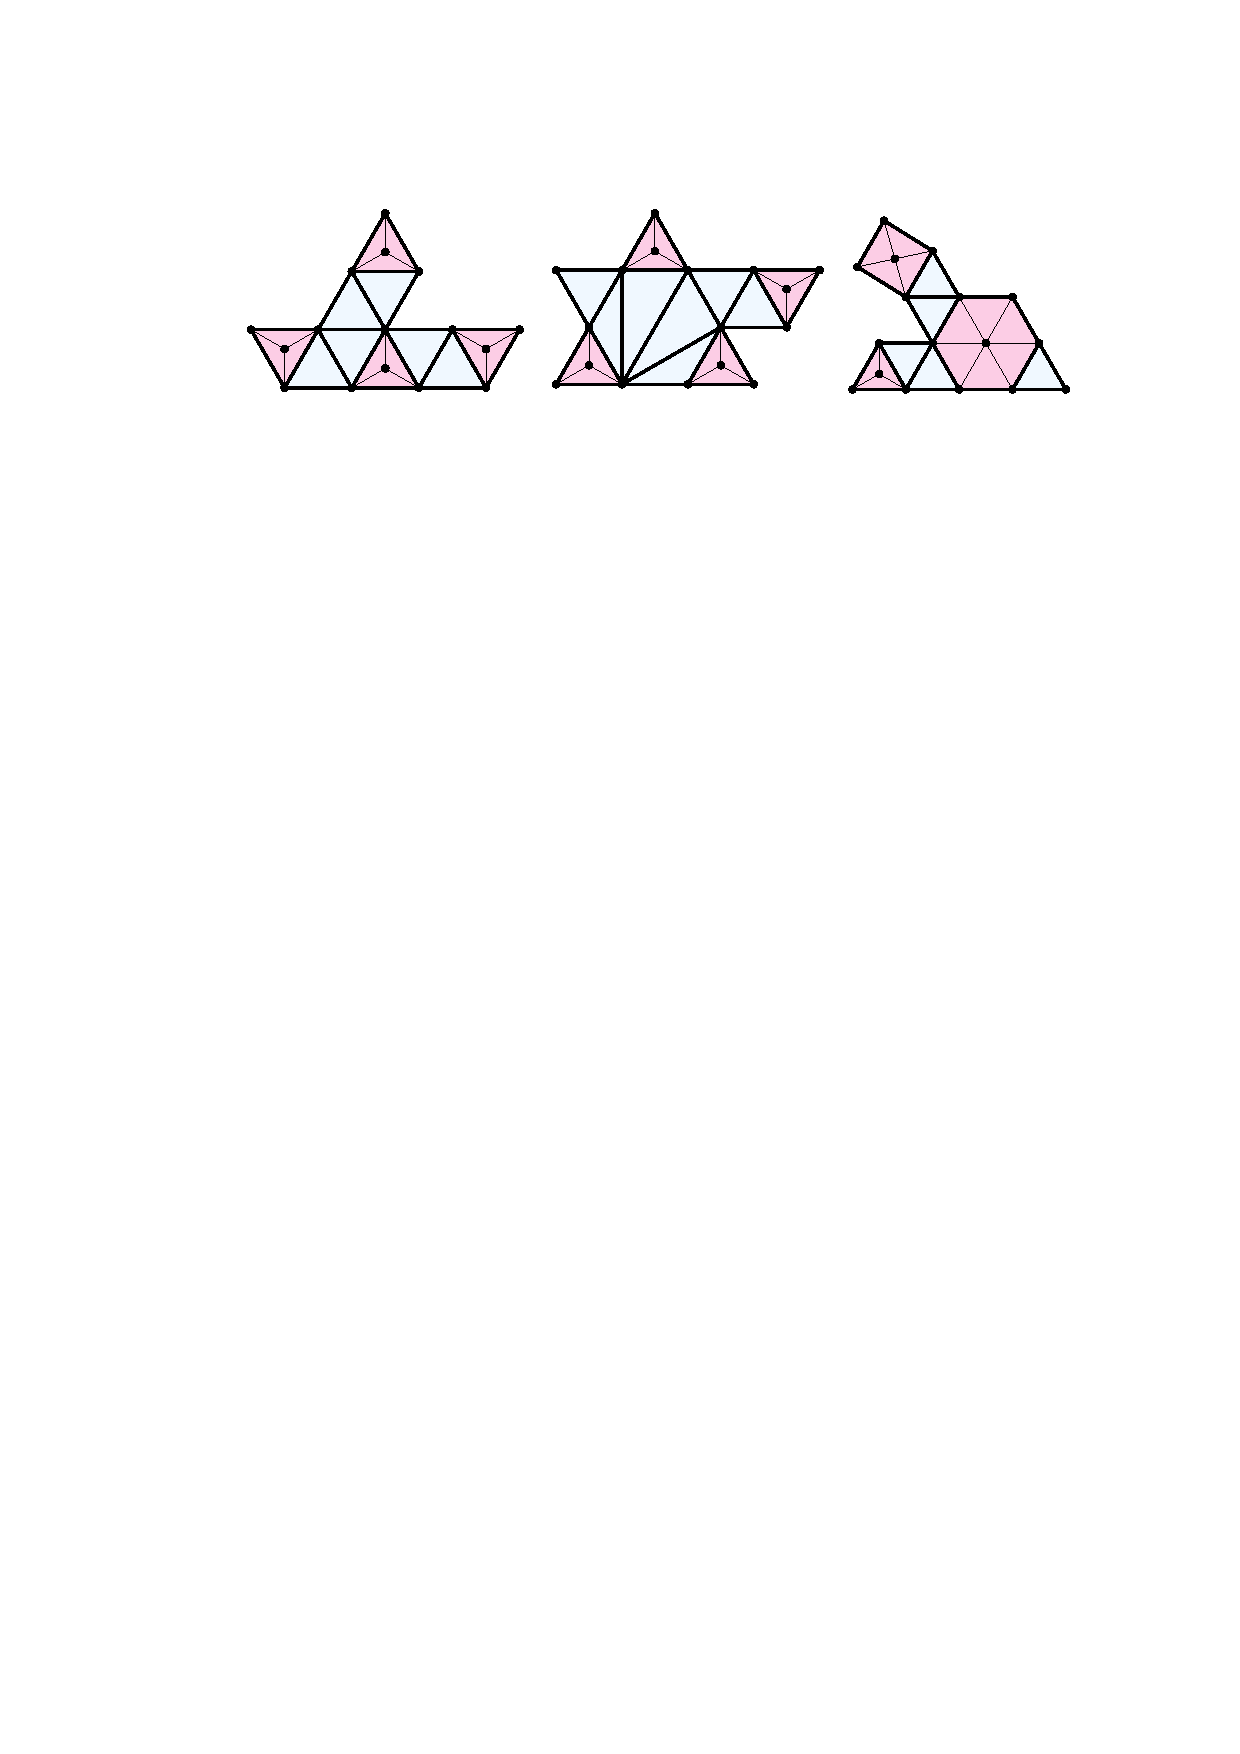
\includegraphics[page=1]{figs/critical} \\
%         % \includegraphics[page=2]{figs/critical} \\
%     \end{center}
%     \caption{Some critical basic graphs. \pat{Add some non-critical examples. These have inner vertices of degree greater than $3$.}}
%     \label{critical_fig}
% \end{figure}

% \begin{lem}\label{base_case}
%     For any basic graph $G$ and any vertex $v\in L(G)$, there exists a dominating set $X\subseteq L(G)$ of size at most $|X|\le |G-L(G)|/2 + |L(G)|/6$.
% \end{lem}

% \begin{proof}
%     Let $H:=G[L(G)]$.
%     Triangulate the face of $H$ that contains $v$ by adding edges incident to $v$ and triangulate the other faces of $H$ by adding edge arbitrarily.  Call the resulting outerplanar graph $H'$.  Create a set $Q$ that contains, for each marked face $f$ of $H$, one triangular face $t$ of $H'$ that is contained in $f$.  Notice that one of the triangular faces in $Q$ contains $v$.  Let $H''$ be the graph obtained from $H'$ by removing any vertex that is not incident on any triangle in $Q$.  
    
%     We claim that $|H''|=3|Q|$.  Indeed, each triangle in $|Q'|$ is incident to exactly three vertices of $H''$ and each vertex of $H''$ is incident to exactly one triangle in $Q'$.  Thus, $|H''|=3|Q'|=3|Q|$.
    
%     Since $H''$ is a subgraph of $H'$, it is outerplanar and therefore has a proper vertex $3$-colouring.  Each triangle in $Q'$ contains vertices of all three colours, so each face in $Q$ contains vertices of all three colours. Take $X$ to be the colour class that contains $v$.  Then 
%     \[  
%         |X| = |Q| = |H''|/3 = |H''|/6 + |H''|/6 = |Q|/2 + |H''|/6 \le |Q|/2 + |H|/6 \enspace . 
%     \]
%     We finish by observing that $|G-L(G)|$ is exactly the number of marked faces in $H$, which is exactly the size of $Q$.
% \end{proof}

% \section{Analysis}

% Now it's time to analyze our algorithm.....

% The key point is that each step $i$ that exposes $k$ vertices of $H$ chooses a vertex $v_i$ with $\deg_{G_i}(v_i)\ge k+2$.

% \end{document}



% % We arrived at $G$ by deleting a sequence $v_1,\ldots,v_r$ of vertices, resulting in a sequence of graphs $G_0,G_1,\ldots,G_r=G$ where $G_i$ is obtained from $G_{i-1}$ by removing $v_i$ to obtain a graph $G_i'$ and then repeatedly removing vertices in $L(G_i')$ having inner degree $0$.  Suppose that $G_i$















% % Of course, this is not always possible and, even if it is, repeatedly choosing a vertex $v$ with $\deg_G^+(v)= 2$ may force us into a situation later when there are no more good choices.  \pat{Can this really happeen?  I don't think so.}





% There is a class of graphs in which we may not be able to reduce the size of $G$ in order to apply induction.  These become the base cases for our induction. Refer to \cref{critical_fig}. Let $G_0$ be an outerplane graph.  A set $Q$ of inner faces of $G_0$ is \defin{good} for $G_0$ if each vertex of $G_0$ belongs to exactly one face in $Q$ and we call $(G_0,Q)$ a \defin{basic pair}.  We say that a graph $G$ is \defin{basic} if $G$ is obtained from a basic pair $(G_0,Q)$ by adding a vertex in each face $f$ of $Q$ and making this vertex adjacent to all vertices of $f$.  We call $G$ the basic graph \defin{described by} $(G_0,Q)$.  A basic pair $(G_0,Q)$ is \defin{critical} if each face in $Q$ is a triangle in which case we call the basic graph $G$ described by $(G_0,Q)$ a \defin{critical basic graph}.

\begin{figure}
    \begin{center}
        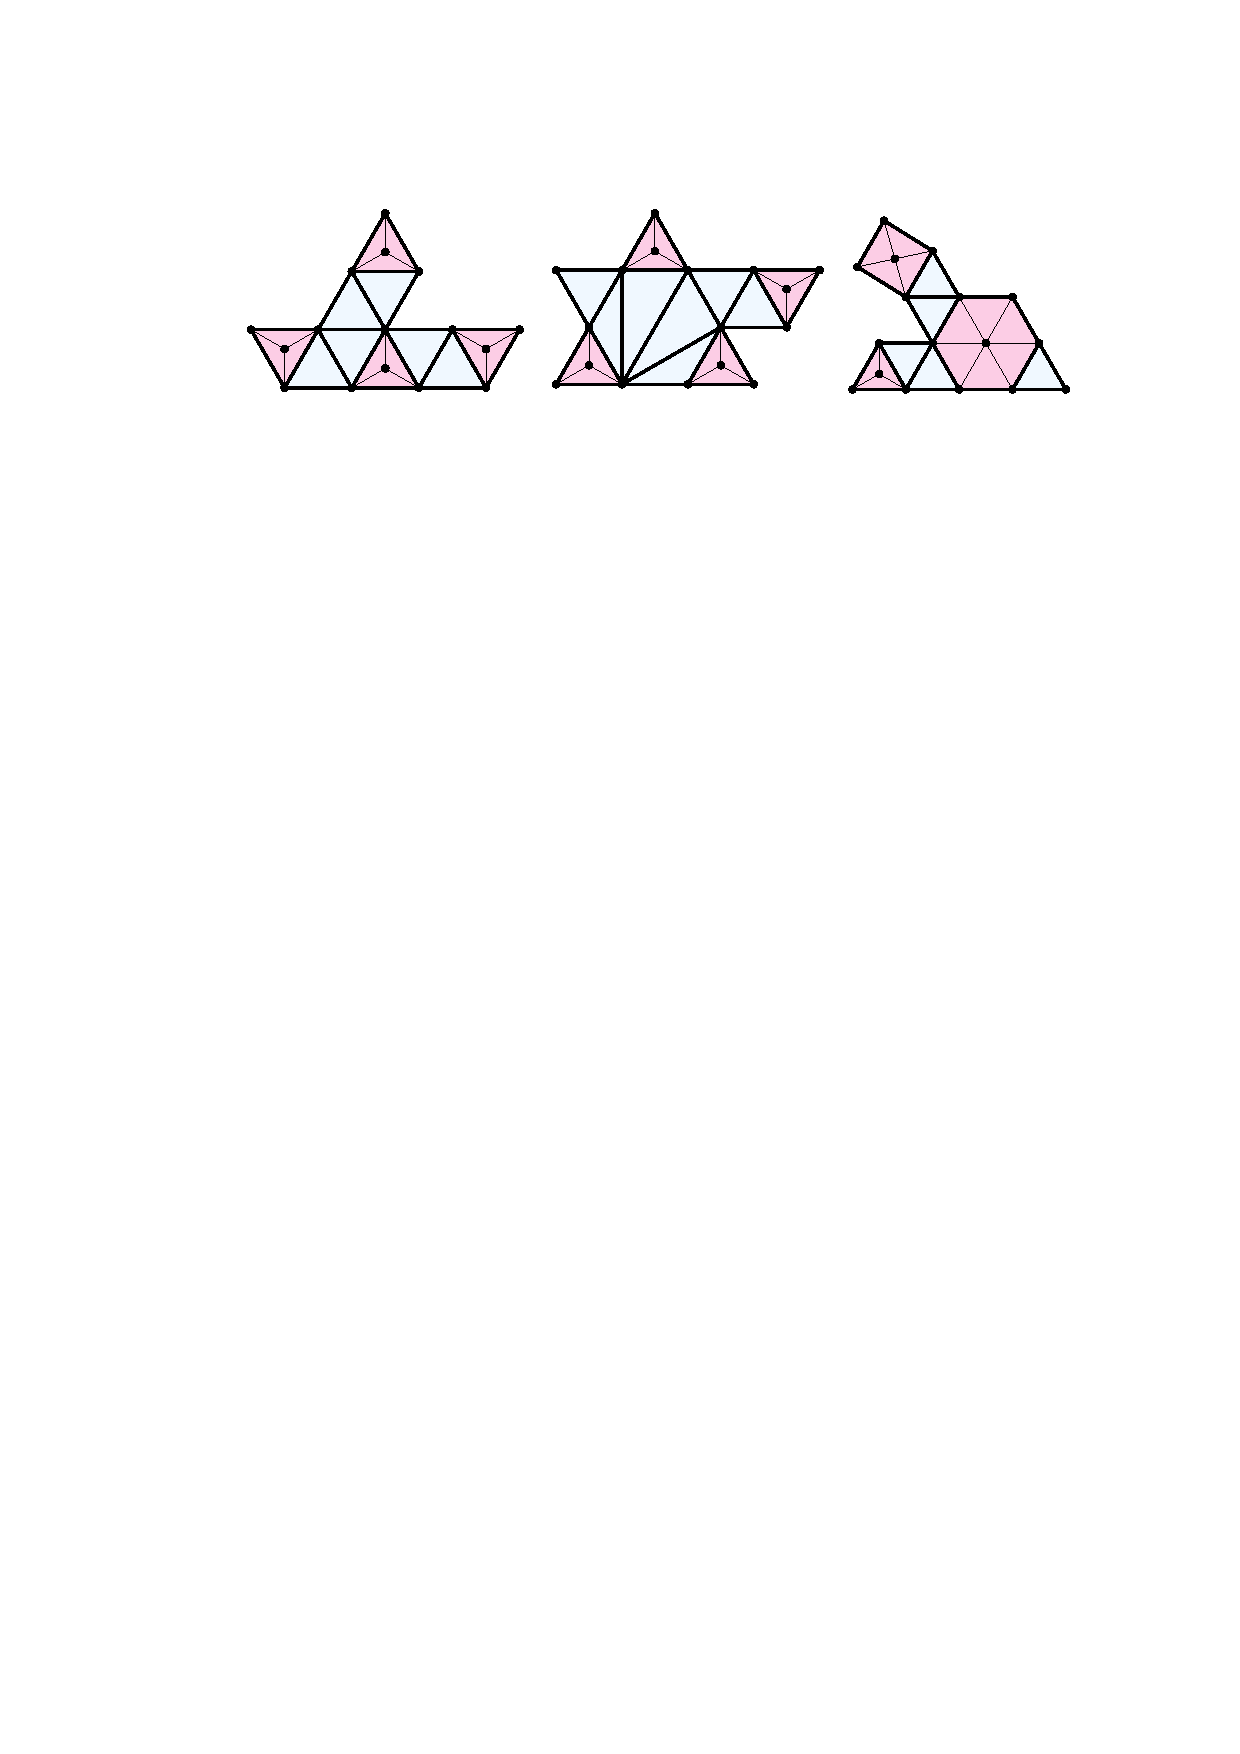
\includegraphics[page=1]{figs/critical} \\
        \includegraphics[page=2]{figs/critical} \\
    \end{center}
    \caption{Some critical basic graphs (top row) and some critical graphs (bottom row). \pat{Add some non-critical examples}}
    \label{critical_fig}
\end{figure}




\subsection{Useless Vertices}

We say that a vertex $v$ in $F(G)$ is \defin{useless} if $\deg^+_{G}(v)=0$.  Suppose $v$ is a useless vertex and let $G':=G-v$.  Then $G'$ has $n':=n-1$ vertices and has the $\ell':=\ell-1$ vertices of $L':=L\setminus\{v\}$ on its outer face.  Since $L'\subseteq L$, $\mu':=\mu(G')=\mu-\mu_{G}(v')\le \mu-1$.  We apply induction to $G'$, to obtain a set $X$ of size at most 
\[
  \frac{n'-\ell'}{2} + \frac{\mu'}{6} = \frac{(n-1)-(\ell-1)}{2} + \frac{\mu-1}{6}
  = \frac{n-\ell}{2}+\frac{\mu}{6} - \frac{1}{6} \enspace ,
\]
which satisfies the requirements of the lemma.  From this point on we assume that there are no useless vertices, so $\deg_G^+(v)\ge 1$ for all $v\in L$.







\Cref{main_result} follows quickly from the following technical lemma:

\begin{lem}\label{main_lemma}
    Let $G$ be a generalized $n$-vertex near-triangulation and let $L:=L(G)$, $n:=|V(G)|$, $\ell:=|L(G)|$ and $\mu:=\mu(G)$.  Then there exists $X\subseteq V(G)$ such that
    \begin{compactenum}
        \item each component of $G[X]$ contains exactly one vertex in $F(G)$; \label{boundary}
        \item each vertex of $G-L(G)$ is either in $X$ or adjacent to a vertex in $X$; \label{dominating}
        \item $|X|\le (n-\ell)/2 + \ell/6$. \label{size}
        \item  $\deg^+_G(v) \ge 2$ for each $v\in X$. \label{no_ones}
    \end{compactenum}
\end{lem}

Before proving \cref{main_lemma}, we first show how it implies \cref{main_result}.

\begin{proof}[Proof of \cref{main_result} assuming \cref{main_lemma}]
    Let $G$ be an $n$-vertex triangulation on $n\ge 4$ vertices.  Then $L(G)$ has size $3$ and $\mu(G)=3$.  Apply \cref{main_lemma} to $G$ to get the set $X$, whose size is at most $(n-3)/2 + 3/6=(n-2)/2$.  Since $n\ge 4$, $V(G)\setminus F(G)$ is non-empty and (\ref{dominating}) therefore implies that $X$ is non-empty and (\ref{boundary}) implies that $X$ contains at least one vertex of $F(G)$.  Since $G[F(G)]$ is a clique, every vertex of $L(G)$ is either in $X$ or adjacent to a vertex in $X$.  Combined with (\ref{dominating}) this implies that $X$ is a dominating set of $G$.  Since each component of $F$ contains a vertex in $L(G)$ and $L(G)$ is clique, this implies that $G[X]$ is connected, so $X$ is a connected dominating set of $G$.
\end{proof}

In the remainder of this section, we prove \cref{main_lemma}.  Globally, the proof is by induction on the number of vertices in $G$.  Throughout this section $L$, $n$, $\ell$, and $\mu$ are used as defined in the statement of \cref{main_lemma}.


\subsection{Boring Vertices}

We say that a vertex $v$ in $F(G)$ is \defin{boring} if $\deg^+_{G-v}(w)\le 1$ for all $w\in N_G^+(v)$.  Suppose $v$ is a boring vertex and let $G':=G-v$.  As with a useless vertex, we can apply induction on $G'$ to get a set $X$ of size at most $\frac{n-\ell}{2}+\frac{\mu}{6}$.  The only danger is if $G[X]$ has a component that does not contain a vertex in $L$.  By (\ref{boundary}), every component of $G[X]$ does contain a vertex in $L':=L(G')$.  But $L'=L\setminus\{v\}\cup N^+_G(v)$ and $\deg^+_{G'}(w)\le 1$ for every $w\in N^+_G(v)$.  Then (\ref{no_ones}) implies that $X\cap N^+_G(v)=\emptyset$, so every component of $X$ must contain a vertex of $L'\setminus N^+_G(v)\subseteq L$ on its boundary, as required.  From this point on, we assume that $X$ contains no boring vertices.  That is, for each $v\in L$, $N^+_G(v)$ contains at least one vertex $w$ such that $\deg^+_G(v)\ge 2$. 

\subsection{Cut Vertices}

Suppose that $G$ contains a cut vertex $v$,  so that $G=G_0\cup G_1$ where $G_0$ and $G_1$ are each non-empty and are vertex disjoint except for their common vertex $v$.  For each $b\in\{0,1\}$, define $n_b$, $\ell_b$, $L_b$, and $\mu_b$ with respect to $G_b$ in the obvious way. 

\begin{compactenum}
  \item If $\deg_{G_b}^+(v)=0$ for some $b\in\{0,1\}$ then $v$ is a useless vertex in $G_b$.  Without loss of generality, suppose $v$ is useless in $G_0$.  Apply the lemma inductively to $G_0-v$ to get a set $X_0$ of size $(n_0-\ell_0)/2) + \mu_0/6 - 1/6$.  Next, apply the lemma to the graph $G_{1}$ to get a set $X_{1}$ of size at most $|X_{1}|\le (n_1-\ell_1)/2 + \mu_1/6$. (Notice that the first graph does not contains $v$ while the second one does.) Since $v$ is a cut vertex, $\mu_{1}=\mu_{G_{1}}(v)\le \mu_G(v)-1$.  This implies that $\mu_0+\mu_1\le \mu-1$.   Let $X:=X_0\cup X_1$.  Then
  \[
    |X| = |X_0|+|X_1| \le \frac{n-\ell}{2}+\frac{\mu-2}{6}
  \]
  
  \item \pat{Continue here, dealing with cases of higher degrees.}Otherwise, since $\deg_{G}^+(v)=2$ it must be the case that $\deg^+_{G_0}(v)=\deg^+_{G_1}(v)=1$.  For each $b\in\{0,1\}$, let $n_b:=|V(G_b)|$, and let $L_b$ be the set of vertices on the outer face of $G_b$.  There are two subcases to consider:
  \begin{compactenum}
      \item At least one of $G_0$ or $G_1$ is a padded basic graph.  Suppose that $G_0$ is.  Apply \cref{padded_basic} to $G_0$ to obtain a dominating set $X_0$ that contains $v$ and has size at most $(n_0-|L_0|)/2+|L_0|/6$. 

      Next apply the lemma to $G_1-v$ to obtain a forest $F_1$ and let $X_1:=V(F_1)$. Then
      \begin{align*}
        |X_1| \le \frac{n_1 - 1 - |L_1|}{2} + \frac{|L_1|}{6}
      \end{align*}
      Since $n_0+n_1=n+1$ and $|L_1|+|L_2|=|L|+1$, this gives
      \[
        |X_0\cup X_1| = \frac{n -(|L|+1)}{2} + \frac{|L|+1}{6}
        = \frac{n-|L|}{2} + \frac{|L|}{6} - \frac{1}{3} \enspace .
      \]

      \item Neither $G_1$ nor $G_2$ is a padded basic graph.  Since $\deg_{G_0}^+(v)=1$ and $\deg_{G_1}^+(v)=1$, this implies that neither of $G_0-v$ nor $G_1-v$ is a padded basic graph.  Applying the lemma to each of these graphs gives sets $X_0$ and $X_1$ of size 
      \[
        |X_0\cup X_1| = \frac{n - 2 - (|L|+1)}{2} + \frac{|L|-1}{6}
        = \frac{n-|L|}{2} + \frac{|L|-1}{6} - 1 \enspace .
      \]
      Now the set $\{v\}\cup X_0\cup X_1$ satisfies the requirements of the lemma.
    \end{compactenum}    
\end{compactenum}



\subsection{Base Cases}

There is a class of graphs in which we may not be able to reduce the size of $G$ in order to apply induction.  These become the base cases for our induction. Refer to \cref{critical_fig}. Let $G_0$ be an outerplane graph.  A set $Q$ of inner faces of $G_0$ is \defin{good} for $G_0$ if each vertex of $G_0$ belongs to exactly one face in $Q$ and we call $(G_0,Q)$ a \defin{basic pair}.  We say that a graph $G$ is \defin{basic} if $G$ is obtained from a basic pair $(G_0,Q)$ by adding a vertex in each face $f$ of $Q$ and making this vertex adjacent to all vertices of $f$.  We call $G$ the basic graph \defin{described by} $(G_0,Q)$.  A basic pair $(G_0,Q)$ is \defin{critical} if each face in $Q$ is a triangle in which case we call the basic graph $G$ described by $(G_0,Q)$ a \defin{critical basic graph}.

\begin{figure}
    \begin{center}
        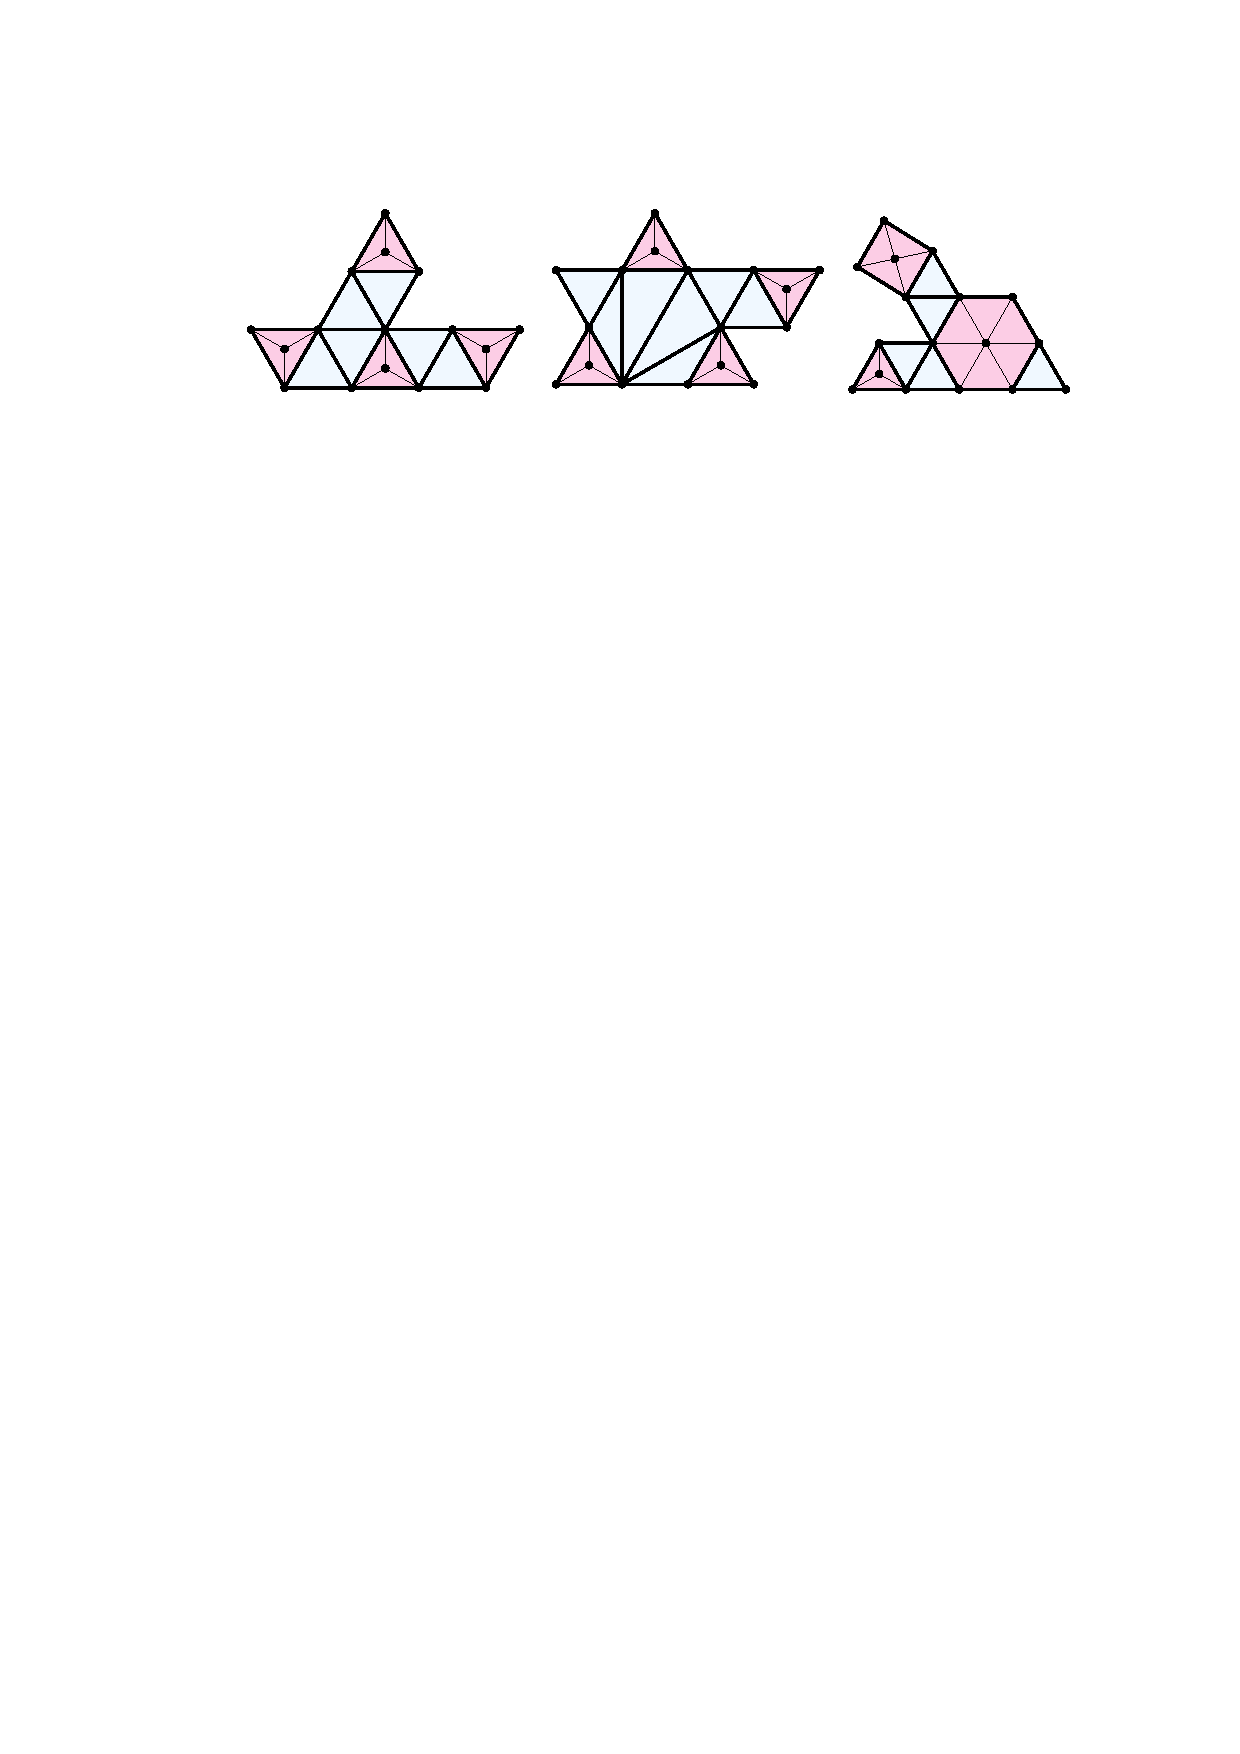
\includegraphics[page=1]{figs/critical} \\
        \includegraphics[page=2]{figs/critical} \\
    \end{center}
    \caption{Some critical basic graphs (top row) and some critical graphs (bottom row). \pat{Add some non-critical examples}}
    \label{critical_fig}
\end{figure}

% \begin{obs}
%     If $(G_0,Q)$ is a basic pair then $|V(G_0)|\le 3|Q|$, with equality if and only if $(G_0,Q)$ is critical.
% \end{obs}

% \begin{proof}
    
% \end{proof}

For basic graphs, we will use the following lemma:

\begin{lem}\label{base_case}
    For any basic pair $(G_0,Q)$ and any vertex $v$ of $G_0$, there exists $X\subseteq V(G_0)$ of size $|X|\le |Q|/2 + |G_0|/6$ such that each face in $S$ contains at least one vertex in $S$.
\end{lem}

\begin{proof}[Proof sketch]
    Triangulate the face in $Q$ that contains $v$ by adding edges incident to $v$ and triangulate the other faces in $Q$ by adding edge arbitrarily.  Call the resulting outerplanar graph $G'$.  Create a set $Q'$ that contains, for each face $f$ in $Q$, one triangular face $t$ of $G'$ that is contained in $f$.  Notice that one of the triangular faces in $Q'$ contains $v$.  Let $Q''$ be the graph obtained from $Q$ by removing any vertex that is not incident to some triangle in $Q'$.
    
    We claim that $|G''|=3|Q|$.  Indeed, each triangle in $|Q'|$ is incident to exactly three vertices of $G''$ and each vertex of $G''$ is incident to exactly one triangle in $Q'$.  Thus, $|V(G'')|=3|Q'|=3|Q|$.
    
    Since $G''$ is a subgraph of $G'$, it is outerplanar and therefore has a proper vertex $3$-colouring.  Each triangle in $Q'$ contains vertices of all three colours, so each face in $Q$ contains vertices of all three colours. Take $X$ to be the colour class that contains $v$.  Then 
    \[  
        |X| = |Q| = |G''|/3 = |G''|/6 + |G''|/6 = |Q|/2 + |G''|/6 \le |Q|/2 + |G_0|/6 \enspace . \qedhere
    \]
\end{proof}

% We say that a basic graph $G$ described by $(G_0,Q)$ is \defin{critical} if $G_0$ is edge maximal and each vertex of $G_0$ is incident to exactly one face in $Q$.  Observe that, if $G$ is critical, then the number of vertices of $G$ is exactly $3|Q|$ since each face in $Q$ is a triangle and each vertex of $G$ appears on exactly one face.  
 
We say that a generalized near triangulation $G$ is a \defin{(critical) padded basic graph} if $G$ is a (critical) basic graph or if $\deg^+_G(v)=2$ for each vertex $v\in F_o(G)$ and $G-F_o(G)$ is a (critical) padded basic graph.



\begin{lem}\label{padded_basic}
    Let $G$ be an $n$-vertex padded basic graph with outer face $F$.  Then, for any $v\in F$, $G$ contains a forest $F$ such that
    \begin{compactenum}
        \item each component of $F$ contains exactly one vertex in $L$; 
        \item each vertex of $V(G)\setminus L$ is either in $F$ or adjacent to a vertex in $F$; 
        \item $|F|\le (n-|L|)/2 + |L|/6$. 
        \item $v$ is a vertex of $F$.
    \end{compactenum}
\end{lem}


\begin{proof}
    If $G$ is a basic graph (without padding) described by $(G_0,Q)$ then apply \cref{base_case}.  Otherwise, if $|F|$ is even, then put every second vertex of $F$ (including $v$) into $X$ and apply induction of $G-F$.  If $|F|$ is odd, then add every second vertex of $F$ to $X$ (including $v$), leaving one edge $xy$ of the outer face of $G$ neither of whose endpoints is in $X$.  Opposite this edge is a face $xyz$ and the vertex $z$ has no neighbour in $X$.  In fact $z$ is the only vertex on the outer face of $G-F$ that has no neighbour in $X$.  Now we apply induction on $G-F$ but make use of the fact that we can choose a vertex $v'$ on the outer face of $G-F$ that must be included in $X$.  In particular, we choose $v'$ to be a neighbour of $z$ on the outer face of $G-F$.  This  ensures that $z$ is adjacent the vertex $v'\in X$.  (Note that in this case, we actually win something, 
\begin{figure}[htbp]
    \begin{center}
        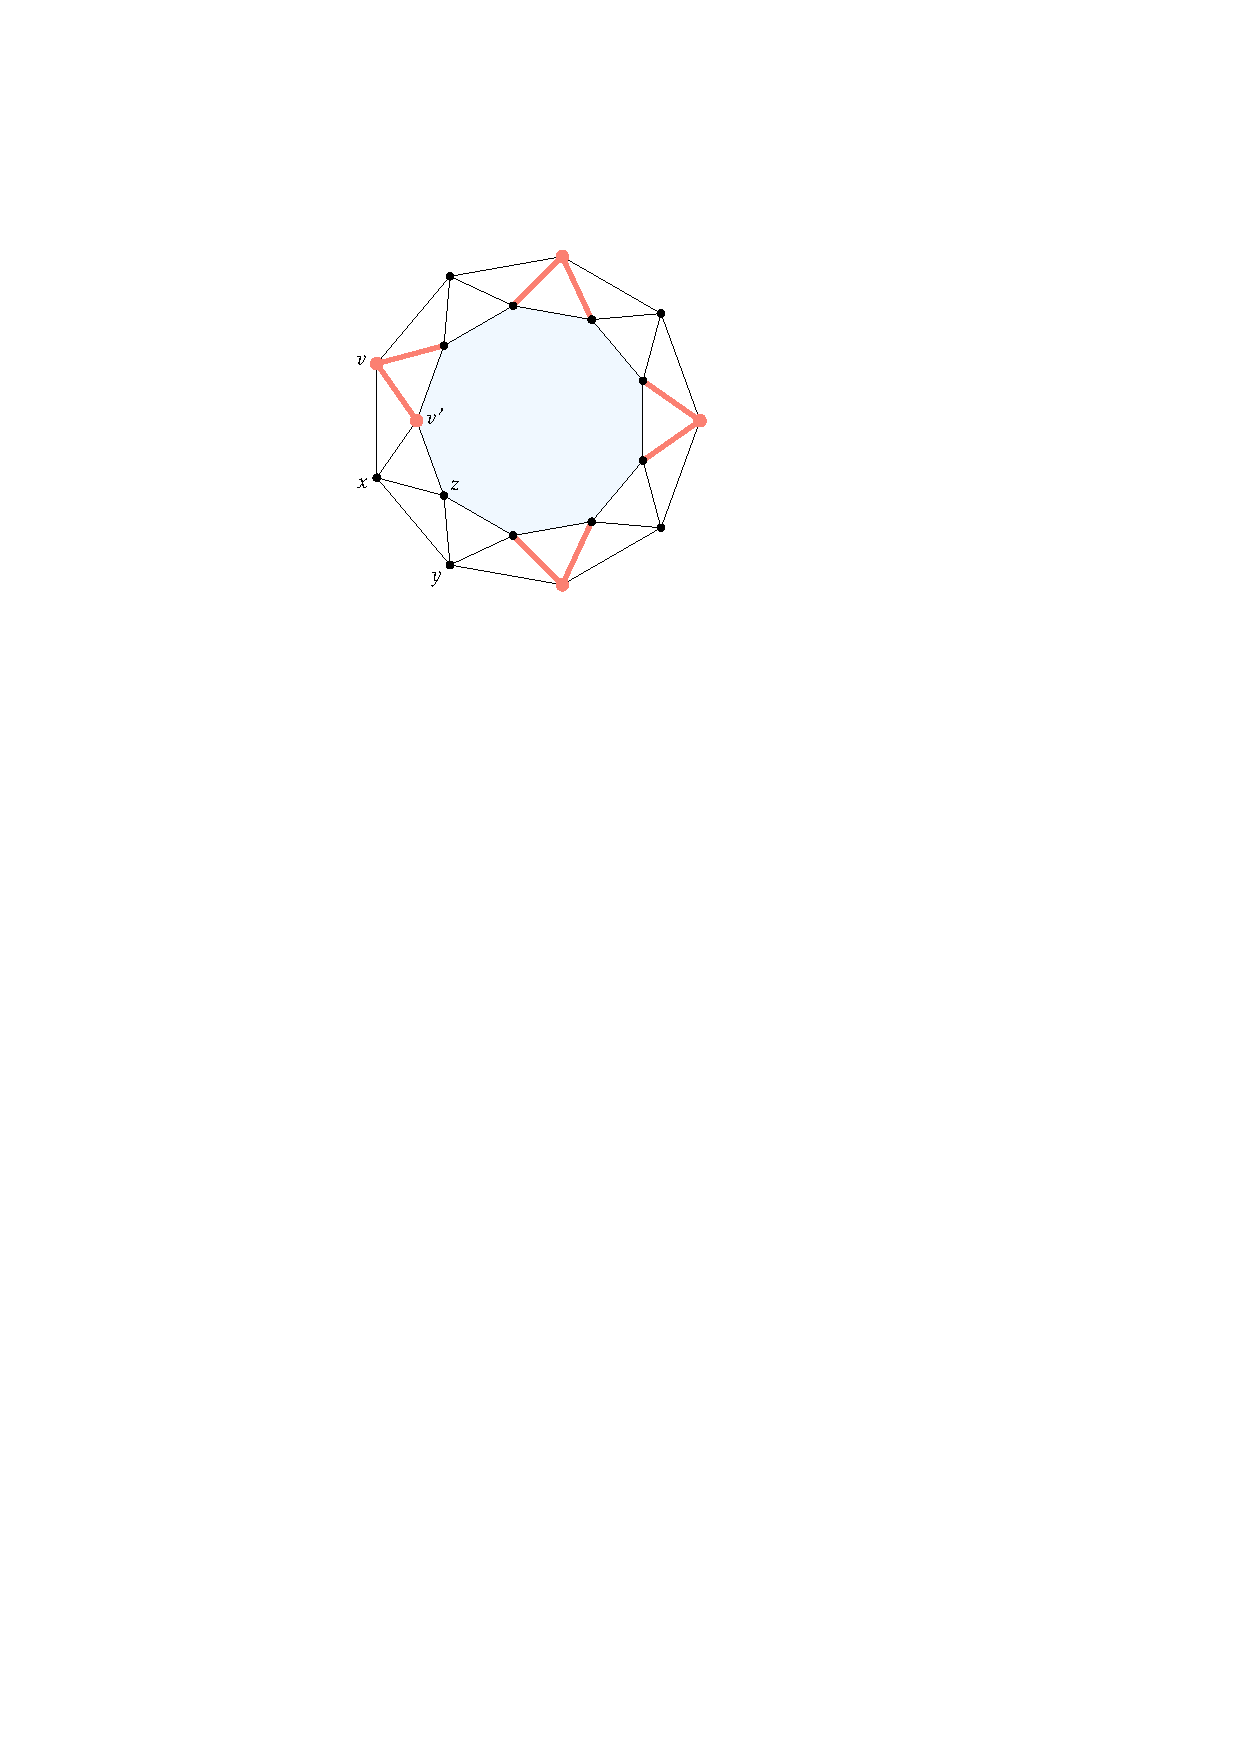
\includegraphics{figs/odd} \\
    \end{center}
    \caption{Dealing with the case where $|F|$ is odd in \cref{padded_basic}.}
    \label{odd_case}
\end{figure}    
\end{proof}






\subsection{No Gains}

For any plane graph $G$ with outer face $F_o(G)$, and any vertex $v$ of $G$, let $N_{G}^+(v)=N_G(v)\setminus V(F_o(G))$ and let $\deg_G^+(v)=|N^+_G(v)|$.  

If $G$ contains a vertex $v$ with $\deg^+_G(v)=0$, we let $G':=G-v$, $n':=n-1$, and $L':=L\setminus\{v\}$.  Observe that $L'$ is the set of vertices on the outer face of $G'$.  Applying induction on $G'$ gives a forest $F$ with    
\begin{align*}
    |F'| 
        % & \le \frac{n'-|L'|}{2} + \frac{|L'|+|L'|\bmod 2}{6} \\
        & \le \frac{n'-|L'|}{2} + \frac{|L'|}{6} \\
        & = \frac{n-|L|}{2} + \frac{|L|-1}{6} \enspace . 
\end{align*}

We now assume that $d_G^+(v)\ge 1$ for all $v\in L$.

\subsection{Some $1$-Gains}

If $G$ contains an edge $vw$ with $v,w\in L$, $\deg_G^+(v)=1$ and $\deg^+_G(w)=2$ then we remove both $v$ and $w$\ldots

\subsection{All $1$-Wins}

If $\deg_G^+(v)=1$ for each $v\in L$, then we appeal to \cref{base_case}.    The graph $G$ is just an outerplanar graph with some stars added to some of its faces.  \pat{If $G$ is critical, then this outerplanar graph is edge maximal and the faces with stars in them partition the vertices.  Then it's clear that every colour class has the same size so we can prescribe that some particular vertex on the outer face be in our solution (this gets used later, when dealing with cut vertices). If $G$ is not critical, then one of the colour classes is smaller and we get our extra $-1/6$ that way.}



\subsection{Big Gains}

If there exist a vertex $v\in L$ with $\deg^+(v)\ge 3$ then let $G':=G-v$, let $n':=n-1=|V(G')|$, and let $L'$ be the set of vertices on the outer face of $G'$.  
Then $|L'|=|L|+\deg_{G}^+(v)-1$.  Applying induction on $G'$ gives a forest $F'$ of size
\begin{align*}
    |F'| 
        % & \le \frac{n'-|L'|}{2} + \frac{|L'|+|L'|\bmod 2}{6} \\
        & \le \frac{n'-|L'|}{2} + \frac{|L'|}{6} \\
        & = \frac{n-|L|-\deg_{G}^+(v)}{2} + \frac{|L|+\deg_{G}^+(v)}{6} \\ 
        & = \frac{n-|L|}{2} + \frac{|L|}{6} - \frac{\deg_{G}^+(v)}{3} \\ 
        & \le \frac{n-|L|}{2} + \frac{|L|}{6} - 1 \enspace . 
\end{align*}
\pat{Argue that if $G'$ is critical then $\deg^+_G(v)\ge 4$, so there is an extra $-1/3$ in the preceding equation. Critical graphs are full of $1$-win vertices.  Before removing $v$, one of these vertices was a $2$-win vertex adjacent to a $1$-win vertex, and we could have gotten rid of it that way, instead.}



% The final inequality requires some explanation.  If $\deg_{G}^+(v)=3$, then $\deg^+_G(v)/3=1$ and $|L'|=|L|$, so $|L'|\bmod 2 = |L|\bmod 2$.  If $\deg_{G}^+(v)\ge 4$, then $\deg_{G}^+(v)/3\ge 1+1/3 > 1+(|L|\bmod 2-|L'|\bmod 2)/6$.

To obtain the forest $F$, we add $v$ to $F'$ and make $v$ adjacent to each vertex in $V(F')\cap N^+_G(v)$.  This gives a forest $F$ of size at most $(n-|L|)/2 + |L|/6$, as required.

We now assume that $d_G^+(v)\le 2$ for all $v\in L$.



\subsection{All $2$-Wins}

The only remaining possibility is that $\deg_{G}^+(v)=2$ for each $v\in L$.   

\subsubsection{Eliminating Cut Vertices}

Without loss of generality, we may assume that $G$ is connected since, otherwise we can apply \cref{main_lemma} to each connected component of $G$.  Suppose now that $G$ contains a cut vertex $v$, so that $G=G_0\cup G_1$ where $G_0$ and $G_1$ are each non-empty and are vertex disjoint except for their common vertex $v$.

\begin{compactenum}
  \item If $\deg_{G_b}^+(v)=0$ for some $b\in\{0,1\}$ then apply the lemma inductively to $G_b-v$ and $G_{1-b}$\ldots

  \item Otherwise, since $\deg_{G}^+(v)=2$ it must be the case that $\deg^+_{G_0}(v)=\deg^+_{G_1}(v)=1$.  For each $b\in\{0,1\}$, let $n_b:=|V(G_b)|$, and let $L_b$ be the set of vertices on the outer face of $G_b$.  There are two subcases to consider:
  \begin{compactenum}
      \item At least one of $G_0$ or $G_1$ is a padded basic graph.  Suppose that $G_0$ is.  Apply \cref{padded_basic} to $G_0$ to obtain a dominating set $X_0$ that contains $v$ and has size at most $(n_0-|L_0|)/2+|L_0|/6$. 

      Next apply the lemma to $G_1-v$ to obtain a forest $F_1$ and let $X_1:=V(F_1)$. Then
      \begin{align*}
        |X_1| \le \frac{n_1 - 1 - |L_1|}{2} + \frac{|L_1|}{6}
      \end{align*}
      Since $n_0+n_1=n+1$ and $|L_1|+|L_2|=|L|+1$, this gives
      \[
        |X_0\cup X_1| = \frac{n -(|L|+1)}{2} + \frac{|L|+1}{6}
        = \frac{n-|L|}{2} + \frac{|L|}{6} - \frac{1}{3} \enspace .
      \]

      \item Neither $G_1$ nor $G_2$ is a padded basic graph.  Since $\deg_{G_0}^+(v)=1$ and $\deg_{G_1}^+(v)=1$, this implies that neither of $G_0-v$ nor $G_1-v$ is a padded basic graph.  Applying the lemma to each of these graphs gives sets $X_0$ and $X_1$ of size 
      \[
        |X_0\cup X_1| = \frac{n - 2 - (|L|+1)}{2} + \frac{|L|-1}{6}
        = \frac{n-|L|}{2} + \frac{|L|-1}{6} - 1 \enspace .
      \]
      Now the set $\{v\}\cup X_0\cup X_1$ satisfies the requirements of the lemma.
    \end{compactenum}    
\end{compactenum}


\end{document}
